\documentclass[a4paper, 11pt]{article}
\usepackage{graphicx, float, url}
\title{Project Deliverable 1\\ High-Level Technical Requirements}
\author{Joshua Frankie Rayo\\ 2011-19612\\ MS Computer Science}
\date{\today}

\begin{document}
\maketitle
\tableofcontents
\listoffigures

\section{Project Overview}
\subsection{Scope}
The purpose of this document is to describe the high level requirements for the Election Management System (EMS), Vote Counting Machine (VCM) and the Optical Mark Reader (OMR).
This documents covers both functional and non-functional requirements of the overall system that should be achieved by the end of the project cycle.

\subsection{Audience}
This high-level requirements document should only be used by members of the Bids and Awards Committee (BAC) of the Commission on Elections (COMELEC), with Ms. Helen G. Aguila-Flores as the Chairperson.
The aforementioned entity will implement and verify the correct functionality of the system.

\subsection{Background}
The COMELEC, through BAC invites interested bidders to bid for the \textit{Lease with Option to Purchase of Election Management System (EMS) and Precinct-Based Optical Mark Reader (OMR) or Optical Scan (OP-SCAN) System} to be used for the \textit{2016 National and Local Elections} with the total \textit{Approved Budget for the Contract (ABC)} of \textit{Two Billion Five Hundred Three Million Five Hundred Eighteen Thousand Pesos (Php 2,503,518,000.00)}.

\subsection{Context}
This document is a requirement for partial completion of CS 260: Advanced Software Engineering course in Department of Computer Science, University of the Philippines Diliman.
This is for academic purposes only.

\subsection{Objectives}
\begin{itemize}
  \item To provide the BAC staff with new system that will implement the necessary requirements for the EMS, VCM and the OMR.
  \item To provide the BAC staff the ability to manage election-related data and generate reports through the EMS.
  \item To provide the BAC staff the ability to consolidate public votes with optimum security and accuracy through the VCM.
  \item To provide the BAC staff the ability to read ballot marks as votes through the OMR.
\end{itemize}


\section{Software Development Plan (SDP)}
\subsection{Overview of Required Work}
The software plan will apply an Incremental strategy to develop and evolve the functional capabilities of the EMS. The "incremental" strategy determines user needs and defines the system requirements, then performs the rest of the development in a sequence of builds. The first build incorporates part of the planned capabilities, the next build adds more capabilities, and so on, until the system is complete. The requirements and constraints of EMS are already explained in section \ref{ems}. All issues concerning cost, schedule and incremental build content must be negotiated with COMELEC.

\subsection{Plans for Performing General Software Development}
\begin{figure}[H]\label{fig:dev}
	\begin{center}
		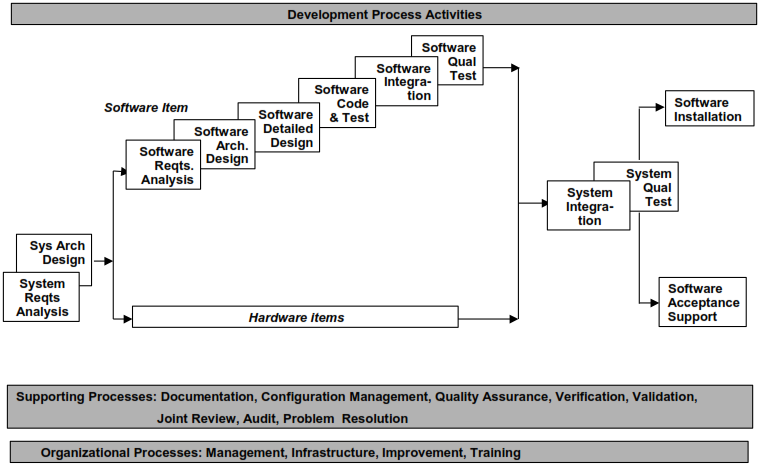
\includegraphics[width=\textwidth]{Picture1.png}
		\caption{Software Engineering Process Model}
	\end{center}
\end{figure}
Section \ref{arch} contains the specific of the web application implementation of the processes in Figure \ref{fig:dev}. The allocation of functional requirements for each build will be negotiated with COMELEC and documented in the Build Plan for each build. The Build Plan will also include build specific acc
eptance criteria and installation/user training requirements. Software design and coding will be performed using an object oriented design approach and generate class and object process interaction diagrams. Artifacts and evidence of results of software development activities will be deposited in Software Development Files (SDFs) and Software Engineering Notebooks (SENs). These artifacts, along with pertinent project references will be deposited and maintained in a Software Development Library (SDL) and made available to support management reviews, metrics calculations, quality audits, product evaluations, and preparation of product deliverables.

Following integration of reusable and new software units, a software Formal Qualification Testing (FQT) will be performed in accordance with processes defined later. A Test Readiness Review (TRR) will be conducted to verify readiness for system level testing.

The development team will prepare a Test Plan (TP) for a system level FQT and execute test cases defined in the implementing Test Description (TD). They will generate Problem/Change Reports (PCRs) to describe software errors uncovered during test results analyses. The developers will do the codes, and testers will do the testing/QA.
The whole system shall be built from scratch. Software reuse is irrelevant as the requirements are very specific.

\subsubsection{Software Development Methods}
The software development will apply the following general methods:
\begin{enumerate}
	\item The development will follow the defined processes documented in Section \ref{plan} to conduct software requirements analysis and manage the Software Requirements Specification (SRS). Express software requirements in language that addresses a single performance objective per statement and promotes measurable verification. Construct a software architecture that will consist of components to be developed. Use an automated data base tool to capture, cross-reference, trace and document requirements.
	\item The developer team and the testing team collaborate during software requirements analysis and then each proceed with separate activities that are intended to ensure the software complies with the detailed software requirement specification. These activities will be addressed separately in Section 5.
\end{enumerate}
\begin{figure}[H]\label{fig:act}
	\begin{center}
		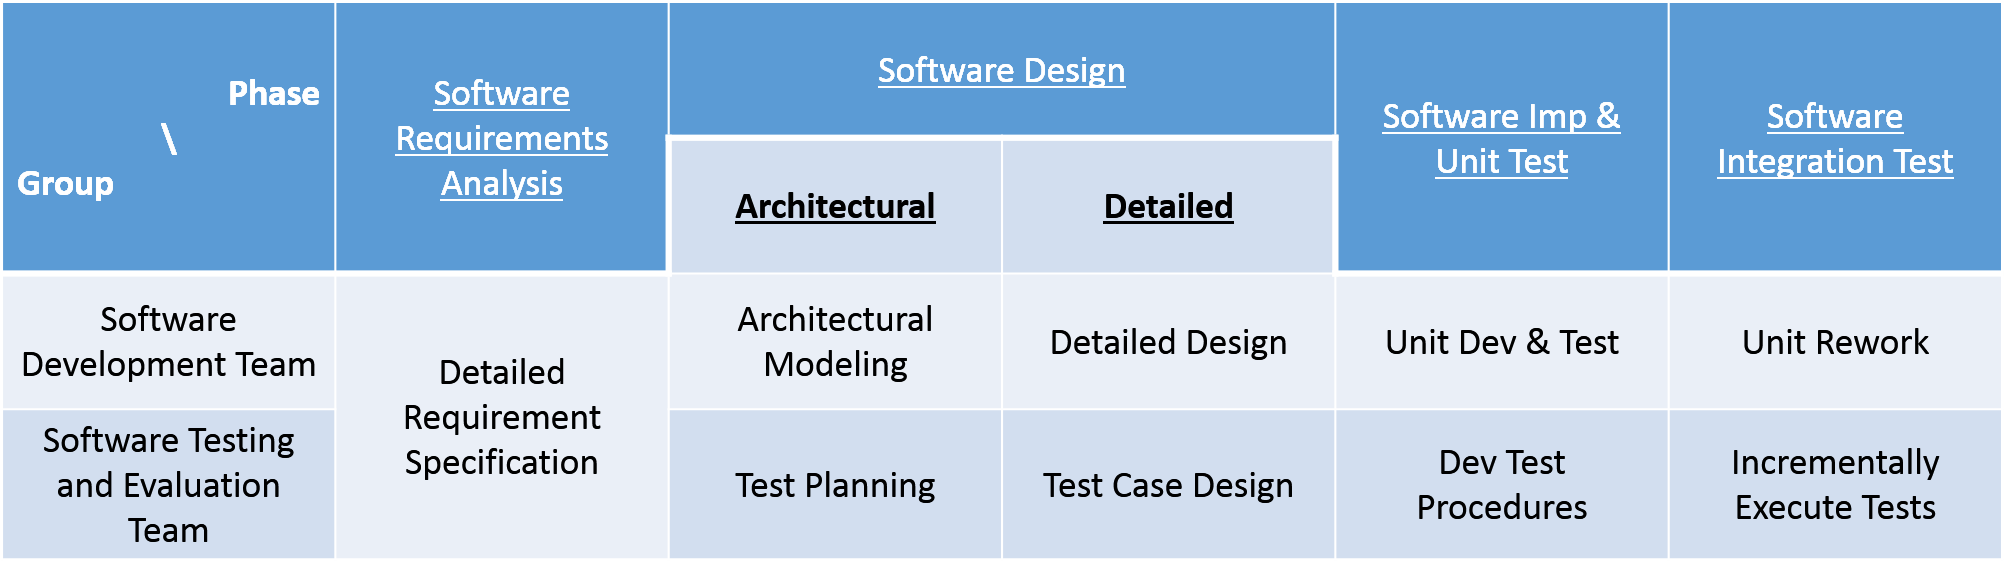
\includegraphics[width=\textwidth]{act.png}
		\caption{Development Activities}
	\end{center}
\end{figure}

\subsubsection{Security and Privacy Assurance}
The system will be subject to product evaluations, quality assurance, and test/evaluation activities conducted to assure that developed software meets the security and privacy requirements imposed by COMELEC.
Software developers, integrators and testers will adhere to security procedures to assure correct access to and handling of classified software, data and documentation. Security and privacy assurance procedures will be reviewed for compliance.

\subsection{Plans for Performing Detailed Software Development Activities}\label{plan}
\subsubsection{Project Planning and Oversight}
This SDP shall be maintained and modified to reflect the current plans, policies, processes, and standards affecting the EMS. It shall be the \textit{Project Manager's} responsibility to keep abreast of industry technology changes and programmatic direction from the \textit{Program Manager} that would require modification of this plan.
\subsubsection{Software Development Planning}
The plan for software development shall employ software engineering 'best' practices in verification and validation, configuration management, peer reviews, project tracking and oversight, and software quality assurance. Trello boards (see \url{http://trello.com}) will be used to develop and maintain the master plan and schedule. In addition, each build will be subject to the planning process described in the figure below and the build's plan will be rolled up into the master project plan. The build project plans will be made available to all participants. The Project Manager will use weekly project-wide meetings to maintain the status of the software project and to resolve any conflicts or changes that might occur. The Project manager will employ a database to record action item assignments, status, and resolutions.

\begin{figure}[H]
	\begin{center}
		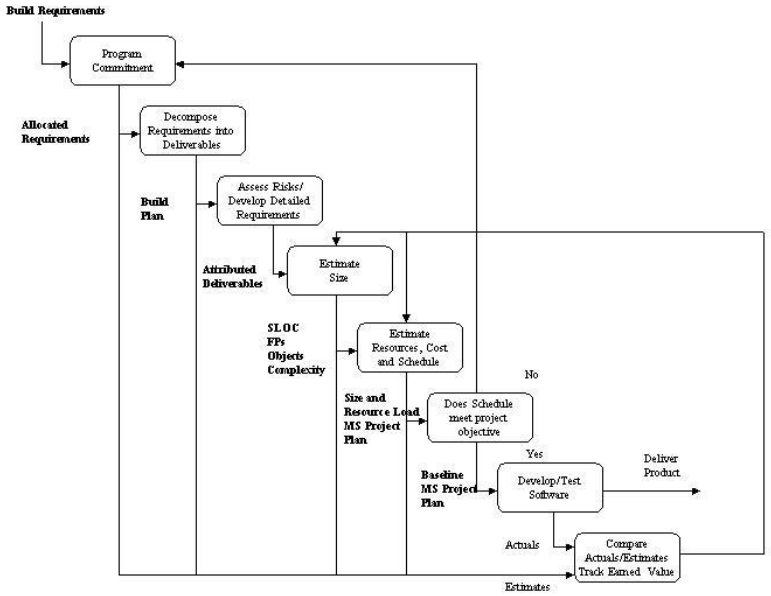
\includegraphics[width=\textwidth]{plan}
		\caption{Project Planning and Oversight Process}
	\end{center}
\end{figure}

\subsubsection{System Planning}
The intent of system test planning is to validate that the system meets its performance requirements. It will be the responsibility of the System Test Manager to direct the development of system test plans and procedures based on the System/Subsystem Specification (SSS), and
conduct the system tests. Section \ref{test} documents the processes for system test planning, test case construction, test procedure development, test conduct, results analysis, test reporting and
participation of the Software Testing Group.

\subsubsection{Software Installation Planning}
Software installation is at the direction of the Project Manager and will be performed according to the procedures referenced in section \ref{install} of this document and as addressed in the Build Plan for each deliverable build.

\subsection{Establishing A Software Development Environment}
This section describe the approach to establish and maintain the physical resources used to develop and deliver the EMS.

\subsubsection{Software Engineering Environment}
The EMS hardware/software development and integration will take place at COMELEC office. The initial phase of software development will take place in the company headquarters, while the hardware integration will take place at COMELEC. The tool sets that will be used on the project consists of the following:
\begin{itemize}
	\item \textbf{Development}: Kali Linux OS, Sublime Text Editor
	\item \textbf{Project Schedule}: Trello
	\item \textbf{Configuration Management}: Git. Repository to be hosted at GitLab
	\item \textbf{Documentation}: Google Drive
\end{itemize}

\subsubsection{Software Test Environment}
The Software Test Enviromnent (STE) for the project will be housed at COMELEC. Many STE components will be the same as those used in the SEE.

\subsubsection{Non-Deliverable Software}
Non-deliverable software shall consist of all the software that is not specifically required to be delivered, but is used in the design, development, manufacture, inspection, or test of deliverable products. It may include but not be limited to the items listed below:
\begin{itemize}
	\item Software used to design or support the design of a deliverable product which may include databases, design analysis, modeling, simulation, digitizers, and graphic plotters.
	\item Software used for in-process testing of deliverable products, or to generate input data or acceptance criteria data for the test program.
\end{itemize}
Non-deliverable software for the XY Project is listed in the table below:
\begin{table}[H]
	\begin{tabular}{l l l l}
		\textbf{Description} & \textbf{Development Phase} & \textbf{Source} & \textbf{Purpose}\\ \hline
		Sublime Text 3 & Development & C & IDE for coding \\
		Ruby On Rails & Development/Testing & Ruby & Web framework \\
		Semantic UI & Development & CSS & Design framework \\
		JQuery & Development & Javascript & Client-side scripting \\
	\end{tabular}
\end{table}

\subsection{Software Design}
The software design approach for the this project will be Object-Oriented Design (OOD). The methodology, definition of terms, and notation for new software design will be based on the Booch Method for OOD. This section describes the software design process and the artifacts produced by this process.

Software design will occur incrementally. A top-level design will be developed during the architectural design phase. During the detailed design phase, the software necessary to meet the capabilities assigned to incremental builds will undergo detailed design to a level sufficient for implementation in support of targeted capabilities.

A software architectural model of XY Project will be placed under developmental configuration management following the top-level design review. Updates and refinements to the model will occur incrementally during detailed design.

\subsubsection{Design Decisions}
Software design decisions will be a continuous effort. The system-wide design principles are listed below:
\begin{itemize}
	\item Establish an initial capability upon which to build future enhancements
	\item Use open system architecture hardware and system software components
	\item Maximize reuse of existing software application packages.
\end{itemize}

\subsubsection{Architectural Modeling and Specification Process}
The Architectural Design step transforms the model created during requirements analysis into the discrete software components that will be required to implement the system software. Detailed design transforms the software component architectural model into an implementation description of the software consisting of Software Units (SUs), their internal data, algorithms, interfaces, and control flow.

The software architectural model of the project will be placed under developmental configuration management following the Formal Inspection of the architectural design. Updates and refinements to the model will occur incrementally during detailed design and the updated model will be placed under developmental configuration management following completion of the Formal Inspection of the detailed design.

\textbf{Inputs}. The inputs for this process are listed below:
\begin{itemize}
	\item Approved system requirements specifications (SRS)
	\item Build plan with documented acceptance criteria
\end{itemize}

\textbf{Process Activity}. The steps needed to complete this process are listed below:
\begin{enumerate}
	\item Review available documentation on requirements, assumptions and constraints.
	\item Formulate and evaluate architectural alternatives.
	\item Select architectural model. Define software components and internal software units, their interactions, data flow and functional processes.
	\item Allocate known requirements to the architectural components.
	\item Identify and select open system architecture hardware and system software components.
	\item Maximize reuse of existing software application packages.
	\item Design and document the initial Graphical User Interface (GUI) and position actions.
	\item Document architectural design in formal design method (e.g . Interaction Diagrams, etc).
	\item Conduct technical review to ensure architectural design meets the requirements allocated to software. Repeat process several times until architectural design meets approval.
	\item Develop initial database scheme to support the system software.
	\item Conduct a technical review of the GUI screen designs to ensure they satisfy system level operational needs and conform to accepted Human Computer Interface (HCI) standards.
	\item Develop a traceability matrix between the components of the architectural design and the SRS.
	\item Provide analysis and comment on architectural model and GUI design.
	\item Conduct Formal Inspection of architectural design, its components/units and their functions, and interaction.
	\item Update the architectural design based on the sum of the accumulated analysis and comments.
	\item Project Manager accepts architectural model and requirements allocation.
\end{enumerate}

\textbf{Outputs}. The outputs for this process are listed below:
\begin{itemize}
	\item Documented and approved architectural design
	\item Documented GUI design
	\item Initial database scheme.
\end{itemize}

\subsubsection{Test Planning Process}\label{test}
The purpose of software test planning is to identify test resources and schedule, and identify tests cases and procedures necessary to the qualification of the developing software in a software test plan (STP).
\textbf{Inputs}. The inputs for this process are listed below:
\begin{itemize}
	\item Approved SRS
	\item Build plan with documented acceptance criteria
	\item Test requirements data base initialized
\end{itemize}
\textbf{Process Activity} The steps to complete this process are listed below:
\begin{enumerate}
	\item Perform analysis of software performance requirements documented in the SRS and identified in Build Plan.
	\item Define test levels for software testing, including general test requirements, test cases (e.g.	stress, erroneous input, maximum capacity, and timing). Define the overall test concept and objectives supported by the defined tests.
	\item Identify the environment in which tests will be conducted. Define plans for implementing and controlling the test environment.
	\item Estimate the personnel and other resources required to support the test concept and objectives.
	\item The Software Project Manager directs Software Test and Evaluation Manager to prepare, conduct, analyze data, and report the results of testing.
	\item Trace software requirements allocated to the test cycle to defined test cases. Verify completeness of requirement's traceability.
	\item Develop a general schedule of defined tests, including time for problem correction and retest.
	\item Draft the STP, following the instructions of the assigned documentation standard. Refine the test requirements database to create structure of test case and procedures with attribution on test characteristics.
	\item The software testing team provide analysis and comment on the STP.
	\item Perform Formal Inspection to ensure that the STP meets the system requirements	allocated to software and is in context with the architectural model and GUI designs.
	\item Revise draft STP to correct discrepancies and incorporate recommended changes.
\end{enumerate}
\textbf{Outputs}. The outputs for this process are listed below:
\begin{itemize}
	\item Approved STP
	\item Test requirements database with attributed test case entries.
\end{itemize}

\subsubsection{Detailed Design}
The purpose of Detailed Design is to incrementally define and describe the software components in terms of their SUs and the internal relationships of those SUs using detailed graphical representation.

If development of detailed design identifies deficiencies in architectural design or software requirements, the Software Developer Team will submit requirement changes and/or update the
developmental architectural model as required.

\textbf{Inputs}. The inputs for this process are listed below:
\begin{itemize}
	\item Approved Software Architectural Design
	\item Approved SRS
	\item Approves GUI design
\end{itemize}

\textbf{Process Activity}. The steps needed to complete this process are listed below:
\begin{enumerate}
	\item Construct graphical representation for each software component detailing the interaction of its SUs.
	\item Add algorithms, data attributes, and operations to each SU.
	\item Draft Software Detailed Design (SDD) document.
	\item Provide traceability matrix from SUs to the parent requirement in the SRS and build plan.
	\item The software testing team provide analysis and comment on the detailed design.
	\item Conduct Formal Inspection of the SDD by component, each component's SUs and their functions and interaction. Repeat process several times until detailed design meets approval.
	\item Update the SDD based on the sum of the accumulated analysis and comments.
\end{enumerate}

\textbf{Outputs}. The output for this process is the SDD containing graphical representation of the detailed design, internal data, and algorithms definitions.

\subsubsection{Test Case Design Process}
The Software Testing Team will design the set of test cases defined in the STP. The design will be in keeping with the overall test concept and objectives of the STP to verify the software meets all performance requirements allocated to the functional components of the architectural design.

\textbf{Inputs}. The inputs for this process are listed below:
\begin{itemize}
	\item Baselined SRS
	\item Baselines STP
	\item Baselined Architectural Design
\end{itemize}

\textbf{Process Activity}. The steps needed to complete this process are listed below:
\begin{enumerate}
	\item Define the test case(s) identified in the draft STD, expressing the purpose and conditions associated with each test case and identify included test procedures. For each test case, perform the following activities:
	\begin{enumerate}
		\item Define the inputs (stimuli to the component under test) required to fulfill the test purpose.
		\item Define the expected results (outputs from the component under test in response to inputs) required to fulfill the test purpose.
		\item Define insertion and extraction methods to/from the component under test. Identify points of data input/output and volumes of data.
		\item Define evaluation criteria for test results analysis. Define ranges of values, capacities, and times for test pass/fail.
		\item Identify test procedure suite (i.e., required discrete procedures).
		\item Identify test environment configuration, interface drivers, database loaders, controllers/monitors, and other test tools to support test case purposes.
	\end{enumerate}
	\item Trace SRS performance requirements to specific test procedures within the test cases.
	\item The software testing group provide analysis and comment on the test case description.
	\item Perform Formal Inspection to ensure that the test case design meets the system requirements allocated to functional component.
	\item Revise draft test case descriptions to correct discrepancies and incorporate recommended	changes.
\end{enumerate}

\textbf{Outputs}. The output from this process is the approved test case descriptions in STD format.

\subsection{Software Implementation and Testing}
The purpose of Software Implementation and Unit Testing is to implement nd test the detailed design for SUs into new code, or as modifications of existing code following documented programming style guidelines.
\subsubsection{Software Implementation}
The purpose of software implementation and unit testing is to create
qualification test ready functional components by implementing and testing each components SUs as identified in the detailed design. This may involve developing new code and/or modifications of existing code, and following documented programming style guidelines.

\textbf{Inputs}. The inputs for this process are listed below:
\begin{enumerate}
	\item Baselines SRS and build plan
	\item Baselined SDD
	\item Approved GUI design
	\item Initial database scheme
\end{enumerate}

\textbf{Process Activity}. The steps needed to complete this process are listed below:
\begin{enumerate}
	\item Review requirements allocated to the SUs, the SDD, and programming style guidelines.
	\item Maintain working source for assigned task within the SDF.
	\item Compile software.
	\item Perform tracing of each SU implementation to the parent software component in the SDD.
	\item Review all inputs and outputs for each software unit. Identify any test drivers necessary to stimulate unit execution, provide inputs, and capture final outputs. Identify all	interfaces to other units and determine if other units are available or if unit stubs must be written.
	\item Identify the various paths that may be taken by the unit (a McCabe complexity analysis tool may be used to determine the unit paths). Identify data variables and conditions that	determine which paths are taken. Identify parameter limits for all input, output, and control parameters. Examine and list all error handling facilities of the units and error conditions.
	\item Identify a set of unit tests to conduct the required testing (path testing, boundary condition testing, and input validation and syntax testing). There should be a test for each path through the unit, to test the upper and lower limits of all parameters, and to test all error conditions (pass and fail). Write step-by-step procedures for each test case.
	\item Document the unit tests in the SDF.
	\item Conduct technical review of each SUs implementation and unit tests. Resolve all comments.
	\item Perform the test in accordance with the unit test plan.
	\item Compare test results with expected results and SU acceptance criteria (e.g., 80\% path test analysis successful). Document the results in the SDF. If discrepancies are found, attempt to determine whether the errors are associated with the software, test/test driver,	or hardware. Rework as required.
	\item The software testing group provide analysis and comment on the content of the SDFs.
	\item The software development team, upon successful completion of the unit test for a software components included SUs, promotes the software component for integration testing, and	submits the software component for developmental CM in the SDL.
	\item Document and report requirement and/or design errors/inconsistencies.
	\item Update metrics information, including defect analysis database.
\end{enumerate}

\textbf{Outputs}. The outputs from this process are listed below:
\begin{enumerate}
	\item Current SDFs
	\item Updated SDL (includes qualified SUs)
	\item Defect database
\end{enumerate}

\subsubsection{Unit Testing}
The purpose of the unit testing is to identify and correct as many internal logic errors as possible. Problems not uncovered by unit testing are, in general more difficult to isolate when uncovered at the integration level. Unit testing will be conducted throughout the implementation process, first as part of the initial development process and later as changes to the unit are made. Unit tests will be repeatable and may be conducted at any point in the implementation process in accordance with the approved unit test plan. For the purposes of unit
testing, a unit is an object. The goal for unit testing by developers is to perform path testing in which every affected branch is navigated in all possible directions at least once and every affected line of code is executed at least once. Unit test drivers and stubs will be developed as
needed and will be placed under CM as part of the overall test utility. All unit test results will be recorded in the SDFs.

\subsubsection{Test Case/Procedure Implementation}
The purpose of this process is to develop detailed steps for controlling tests, injecting inputs, recording results, and comparing actual to expected results.

\textbf{Inputs}. The inputs for this process are listed below:
\begin{enumerate}
	\item GUI screen and/or operator manual
	\item Test case designs
\end{enumerate}

\textbf{Process Activities}. The steps needed to complete this process are listed below:
\begin{enumerate}
	\item Review software GUI and/or operator manuals to identify methods of operator input, use of simulator/emulator tools, and software data recording.
	\item Define and document detailed test procedure steps for providing inputs for test cases.
	\item Prepare input data files to provide test stimuli. Prepare operator logs for the component	under test as well as the test environment.
	\item Define evaluation steps for conducting post-test analysis and comparing actual and expected test results.
	\item Define and document the test procedures in the STD following the instructions of the	assigned documentation standard.
	\item Develop test harness with automated test procedures and test
	result analysis.
	\item Trace specific test case procedures to requirements allocated to parent test case.
	\item The software testing group provide analysis and comment on the on the test procedures.
	\item Conduct a technical review to verify consistency of the test procedures (or test harness/procedures) with the test case descriptions, the STP, baselined requirements, and planning documents. Recommend revisions, as appropriate.
	\item Revise draft STD (or test harness/procedures) to correct discrepancies and incorporate recommended changes to test case definitions and test procedures.
\end{enumerate}

\textbf{Outputs}. The outputs from this process are listed below:
\begin{enumerate}
	\item Baselined test procedures
	\item Test data files compiled
\end{enumerate}

\subsection{Unit Integration and Testing}
The purpose of integration and test is to incrementally integrate SUs into larger software components, and components into a complete system. Testing is performed to validate each component's ability to meet its stated requirements and to ensure interoperability of the major
software components.
Integration continues until all software components are integrated with the system-level hardware suite into a single functioning system.

\textbf{Inputs}. The inputs for this process are listed below:
\begin{enumerate}
	\item Updated SDL (includes qualified SUs)
	\item Baselined STD (includes execution ready test cases with included test procedures)
	\item Integration test report form
	\item P/CR forms
	\item Test drivers and test inspection tools as required by testing
\end{enumerate}

\textbf{Process Activities}. The steps needed to complete this process are listed below:
\begin{enumerate}
	\item Software Testing Group reviews the Build Plan and schedule, the list of	software units/components to be included in the build, and the results of any previous	integration tests to determine the software and software fixes to be tested. Determine a set of test cases to be used to test the build.
	\item For the requirements identified for the build, develop an integration test plan. The integration test plan should identify the sequence of SU and component integration, traceability to the requirements to be validated by the test, test tools and drivers to be used, and the applicable test cases including procedures for conducting the test and	analyzing the results. Document the integration test plan.
	\item Perform a Technical Review of the integration test plan and resolve all comments.
	\item Software Testing Group places the integration test plan under developmental configuration control.
	\item Software Testing Group requests and receives increment build, installs it in the integration test area.
	\item Conduct the test in accordance with the integration test plan procedures. Record test	results as they are observed.
	\item Perform any required post test analysis or data reduction to determine pass/fail criteria as	specified in the integration test plan.
	\item Compare test results with expected results. If discrepancies are found, attempt to determine whether errors are associated with the software, test/test driver, or hardware.
	\item Document all test results using the project integration test report form. This report should	contain all data recorded from test tools, test results, and deviations from the test plan.	Document any problems detected on a P/CR form. Document requirements satisfactorily tested in the test report.
	\item Determine if another incremental build is required. If not proceed to next step.
	\item The software testing group provide analysis and comment on the on the test results.
	\item Software Testing Manager reviews the integration test report and any P/CRs for accuracy and thoroughness. File the test report in the project history file in the document library and submit a copy of the test report and P/CRs to the Software Development Manager for review and analysis.
\end{enumerate}

\textbf{Outputs}. The outputs from this process are listed below:
\begin{enumerate}
	\item Updated SDFs
	\item Updated SDL (i.e., source code and test procedures)
	\item Project History FIle updated with test results
	\item P/CRs submitted for all detected problems
\end{enumerate}

\subsection{System Qualification Testing}
System Qualification Testing (SQT) consists of complementary and progressive test phases. A single STP will be generated to address the planning for all levels of software SQT. A STD will be generated for each CSCI component, documenting the test procedures to be run to verify
each requirement in the SRS for that component. A cross reference matrix will be provided, using the project wide requirements traceability database, to document the test or tests that satisfy each SRS requirement.
The System Qualification Testing (SQT) test will be used to validate the entire systems performance. The System Qualification Testing (SQT) is the client's approved and witnessed series of tests that demonstrate compliance with the requirements set forth in the SSS. The SQT is the acceptance mechanism for the developer's compliance with the terms of tasking by the client.

\subsubsection{Independence in System Qualification Testing}
The SQT shall be accomplished by the Software Testing Team. This is done to ensure that the product accepted by the government meets all system requirements. The client may approve on a case-by-case basis the use of the developer's test staff as SQT testers. However, the conduct of these tests shall remain the responsibility of the Software Testing Team.

\subsubsection{Testing on the Target Computer System}
The target computer system shall be used for all SQT testing. In the event that commercial equivalents are the only system available, the commercial equivalent system shall has the same functional characteristics as the Target Computer System. If the systems are not equivalent, then the follow-on tests will include a test sample of those procedures that could not be run on the Target Computer System.

\subsubsection{Perparing for System Qualification Testing}
SQT will be conducted at the System Test Organization facilities. Following SQT, the program then proceeds to a series of Demonstration Tests (DTs). An Operational Evaluation (OPEVAL) may or may not be conducted based upon the changes to the System Baseline. Since tests
following SQT are performed by external agencies, the processes for these tests have not been discussed.

\subsubsection{Dry Run of System Qualification Testing}
The system test procedures will be reviewed and approved prior to conduct of the SQT. This will allow the developers and testers an early view into problems and issues that might not otherwise be revealed until system testing.

\subsubsection{Performing System Qualification Testing}
The SQT is intended to verify program performance for the project and those requirements specifications referenced from the SRS. The test will include all functional areas and interfaces to verify the functionality of a totally integrated program. Program reliability will be evaluated during independent functional and simultaneous operations, and in light and dense tactical environments. All functions and subsystem interfaces will be independently tested in a systematic manner. Approved test procedures will be developed to allow for repeatability of tests and to facilitate performance analysis. System performance will be visually analyzed, augmented by automated data collection, and results will be recorded by test personnel.

SQT componenets and objectives are listed below:
\begin{itemize}
	\item \textbf{Functional Tests}. Functional Tests comprise two parts: Functional Operability Testing	(FOT) and Functional Stress Testing (FST). FOT and FST test the functional	requirements and the functional stress requirements of the SRS. FOT and FST are	combined within a single set of procedures.
	\item \textbf{Interface Validation Tests (IVT)}. IVTs comprise three parts: Interface Message Tests (IMT), Interface Recovery Tests (IRT) and Interface Stress Tests (IST). These three components test all interface messages, software recovery from interface protocol errors,
	and software response to interface stress, respectively. All IVTs are run with simulators, and to the degree feasible, will be conducted prior to SQT.
	\item \textbf{Regression Tests}. Regression tests are run to verify that program changes implemented following the beginning of SQT testing have not introduced program regression. System tests including a casualty test, is included in the Regression Test set.
	\item \textbf{Single Unit Tests}. Single Unit Tests are performed for each of the XY Project functional areas to validate the program operation individually in a one-on-one link.
	\item \textbf{Multiple Unit Tests}. Multiple Unit Tests are performed simultaneously for all the functional areas to validate the program operation in a multi-unit environment.
	\item \textbf{Stress and Endurance Test}. The Stress and Endurance Test is designed to satisfy the	stress and endurance requirements for critical computer programs. Three periods of maximum stress are distributed throughout a 25 hour period. The program must operate continuously for 25 hours without resulting in a Priority 1 or 2 P/CRs to pass this test.
	\item \textbf{P/CR Correction/Closure Tests}. These tests are executed to verify fixes to problems and to concur with the decision to close.
\end{itemize}
Specific SQT requirements and processes will be specified in the STP.

\subsubsection{Revision and Retesting}
The Regression Test (RT), a set of high level tests, will perform a representative sampling of critical project functions. It will run against a newly delivered operational program during SQT to examine the possibility of regression between the new and previous program versions.
The RT is intended to serve as "system checkout" and should retain a measure of simplicity to ensure that results may be compared from one run to the next. Requirements for this test will be derived from mission-critical functions and casualty requirements identified in the SSS. Specific mission-critical functions are chosen which ensure that failure among them does compromise the overall effectiveness of the XY Project. Testing will be done in a laboratory environment.

\subsubsection{Analyzing and Recording System Qualification Test Results}
Test procedures shall be prepared for each event to be tested in SQT and shall contain clear identification to link it to its particular level of test, as well as to define test objectives. These test procedures shall contain the expected results, a pass/fail notation, and a summary, if
applicable. Evaluations of test data shall provide the basis for a pass/fail determination leading to eventual acceptance or non-acceptance of the program. Problems in either software or design documentation or user manuals shall be documented as a P/CR.

A P/CR is a report describing an existing problem in a computer program or its support documentation. Some P/CRs may, in fact, report a design enhancement rather than a design problem, in which case that PR will eventually be closed-out by submission of an ECP. The P/CRs database contains the following kinds of data: P/CR name, P/CR number, P/CR
description, a category specification, a severity specification, and a process state status code. In addition, the P/CR database incorporates a routing system to direct the handling of each P/CR from station to station such as entry, analysis, approval, design, code, test, acceptance, and closure. The P/CR database program retains comments generated by each station as it advances through the route. The P/CR database program generates a variety of reports by selected category
in specified order.

\subsection{Preparing For Software Use}\label{install}
The software developer team is responsible for correctly packaging the software consistent with the Build Plan and according to the documented processes.

\subsubsection{Preparing the Executable Software}
The executable software will be prepared for each user site, including any batch files, command files, data files, or other software files needed to install and operate the software on its target computer(s). The result is included in the executable deliverable portion of the Program Package (PP) as documented in the Build Plan.

\subsubsection{Preparing User Manuals}
User Manuals will be prepared by the Software Development Team and validated by the Software Testing Team. The Software Librarian will baseline the User Manuals, and provide copies as part of the deliverable Program Package (PP).

\section{Election Management System (EMS)}\label{ems}
The EMS shall be a single integrated system where all functionalities are available from one user interface only. The modules stated below serve as the functional requirements of this particular system.
\subsection{System Administration Utilities Module}
This module shall be used in managing user accounts, rights and privileges, system monitoring, audit log files monitoring and backup files generation, among others.
\begin{itemize}
	\item Require authorization and authentication of all users with unique usernames and user-modifiable passwords with multiple user access levels
	\item Access of EMS shall be from the client-side only
\end{itemize}
The EMS shall employ three levels of user access, as follows:
\begin{itemize}
	\item \textbf{Regular} - basic operational roles such as generation of approved configuration files, VCM usernames and passwords, viewing of EMS data
	\item \textbf{Intermediate} - correction of imported data, approval of configuration files
	\item \textbf{Administrator} - reference file management, data import, assigning and revoking of user rights and privileges
\end{itemize}
User privileges are different for each user access. Addition of selected user rights and privileges from other user access levels are also allowed.
\subsubsection{Record Management Functionalities}
Based on user privileges, the EMS should be able to deliver these functionalities:
\begin{itemize}
	\item View and print records
	\item Edit and update records
	\item Delete records
	\item Create VCM configuration files, usernames and passwords, ballot faces and other requirements stated below.
\end{itemize}

\subsection{Pre-election Data Management Module}
This module shall be used in managing all data to be used for election purposes, including data import of election data files from existing COMELEC software applications, such as the COMELEC existing EMS, Candidate Profile System (CPS), and the Voter Registration System (VRS), among others. Specific features will be the following:
\subsubsection{Data Import}
The EMS shall be capable of importing pre-election data from existing COMELEC applications for information on candidates, voting jurisdictions, geographical subdivisions, among others, as part of its data management capabilities, together with the following additional functionalities:
\begin{enumerate}
	\item Managing pre-election data by direct entry.
	\item Verification and validation of the integrity and accuracy of data before allowing data import.
	\item Displaying the results of data import and its statistical information, with options for filtering display based on data fields.
	\item Accommodate data structures of COMELEC MySQL and CSV files for data import.
\end{enumerate}
Importing data shall commence even without manually dividing the files into small parts. Imported data shall not be modified.

\subsection{Election Configuration Files Management Module}
This module shall automatically generate location-specific configuration files for each VCM to restrict the votes that can be accepted and the results to be generated by each machine.
\subsubsection{Configuration Settings}
The configuration file shall include the following information:
\begin{itemize}
	\item Date and title of elections
	\item Precinct of assignment
	\item Region, province, city or municipality
	\item Post or embassy
	\item Barangay and voting center
	\item Candidate information
	\item Digital certificates
\end{itemize}
The EMS shall allow the configuration of the following settings:
\begin{enumerate}
	\item Number of security keys and users that need access the VCM.
	\item Transmission destination of each position in the VCM.
	\item Enabling or disabling the vote verification feature of VCM that displays a message indicating the affected position and candidate when an ambiguous mark is encountered in the scanned ballot.
\end{enumerate}
Furthermore, the EMS keeps track the number of time a specific precinct configuration file has been programmed in a memory card that shall be recognized by the OMR system upon each start up and then recorded in its audit log.


\subsection{Ballot Definition Management Module}
This module shall be used in managing the generation of the ballot faces that has the following functionalities:
\subsubsection{Ballot Design}
\begin{enumerate}
	\item Automatic creation and preview of ballot faces for each VCM for verification purposes
	\item Generate ballot face for each voting jurisdiction with a common set of candidates from the national level down to the city, municipal level or councilor district level
	\item Creation of unique identifier for each clustered precinct
	\item Customization of final ballot design and layout
	\item Provision of Arabic translation of the title of the offices to be voted for, in addition to the English titles
	\item Assign unique ballot ID for each face
	\item Verify if the positions of the ovals and the security markings on the ballot are correct
	\item Handle all lengths of candidate names without truncating it, and display in the ballot accordingly
	\item Export the ballot face to printable formats
	\item Accommodate at least 350 candidate names including the positions on each side of the face with Arial font face size 10.
	\item Designate physical space for security markings specified by COMELEC, National Printing Office (NPO) or Bangko Sentral ng Pilipinas (BSP) which may not be machine-detectable
\end{enumerate}
\subsubsection{Ballot Printing}
\begin{enumerate}
	\item Export the ballot face to any printable format
	\item Generate one-sheet paper ballots per voter, based on the number of registered voters
	\item Generate machine-readable information that shall identify the ballot jurisdiction codes and its ballot code.
\end{enumerate}

\subsection{Machine Configuration Management Module}
This module shall be used in managing configurations relevant to the VCM.
\begin{enumerate}
	\item Customize the position and time of displaying hash code for the system generated by a cryptographic hash function
	\item Print the particular hash code on all reports generated by the system
\end{enumerate}
Separate application that extracts the hash code for the EMS and validating its integrity shall be provided.

\subsection{Election Data Report Format Management Module}
This module shall be used in managing report formats relevant to election results.
The EMS shall provide a functionality for the creation of report templates that will be generated by the VCM:
\begin{itemize}
	\item Initialization Report
	\item Election Returns (ER)
	\item Statistical Reports regarding
	\begin{itemize}
		\item Ballot faces per date, with summary and detailed listing
		\item Machine configuration files per date for all machines, with summary and detailed listing
		\item Machine usernames and passwords
		\item Multi-level lists of voting jurisdictions
		\item Elective positions per voting jurisdiction
		\item List of candidates per position per voting jurisdiction
	\end{itemize}
	\item Electronic Transmission Report
	\item Audit Log Report
\end{itemize}
Furthermore, additional requirements are necessary for managing the report formats:
\begin{enumerate}
	\item Modification of the title of report, entries, contents and their corresponding positions
	\item Importing report templates from MS Word, ODF and plain text files
	\item Inclusion or exclusion of data fields in the report templates
\end{enumerate}

\subsection{EMS Graphical User Interface}
The EMS shall be easy to use and operate with the use of graphical user interface, with the following requirements:
\begin{enumerate}
	\item On-screen messages and instructions that can be modified with the system
	\item Built-in user manual which shall be accessible from a Help menu that provide instructions on how to operate the system. The user manual shall contain complete, accurate and understandable information and instructions
\end{enumerate}

\section{Proposed System Architecture for EMS}\label{arch}
The Election Management System will be implemented in a web-based application to answer the problems of portability and interoperability.
\subsection{Web Application Specifications}
The web application shall be of the following specifications:
\begin{itemize}
	\item Can be accessed through all kinds of electronic devices with Internet access such as desktops, laptops, tablets, smart phones and the like
	\item Built with Ruby On Rails as the back-end web framework and MySQL as the database
	\item Built with Semantic UI and JQuery as the front-end web framework for the GUI and design responsiveness to support screen sizes of different devices
	\item Hosted in a web sever from GoDaddy to eliminate web server maintenance tasks, as they will do this
\end{itemize}
\subsection{System Modularization}
\begin{figure}[H]
	\begin{center}
		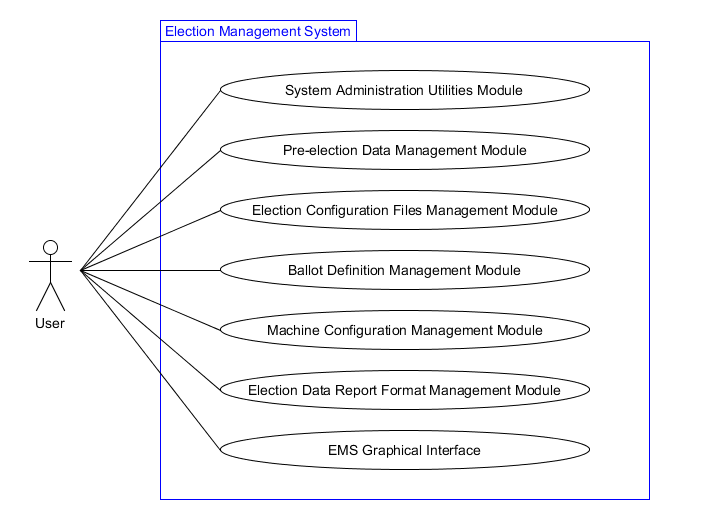
\includegraphics[width=\textwidth]{mes}
	\end{center}
\end{figure}
The EMS shall be divided into five different modules for easier understanding of the system, as well as the use case diagrams to further illustrate the flow of the system.
\subsubsection*{System Utilities Administration Module}
\begin{figure}[H]
	\begin{center}
		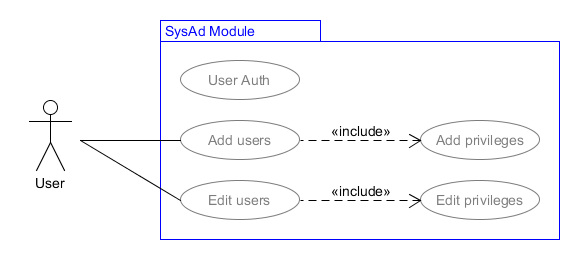
\includegraphics[width=\textwidth]{sysad}
	\end{center}
\end{figure}
\subsubsection*{Pre-Election Data Management Module}
\begin{figure}[H]
	\begin{center}
		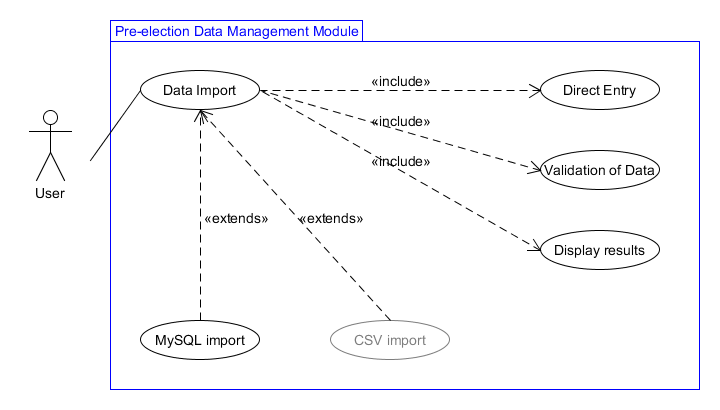
\includegraphics[width=\textwidth]{predata}
	\end{center}
\end{figure}
\subsubsection*{Election Configuration Files Management Module}
\begin{figure}[H]
	\begin{center}
		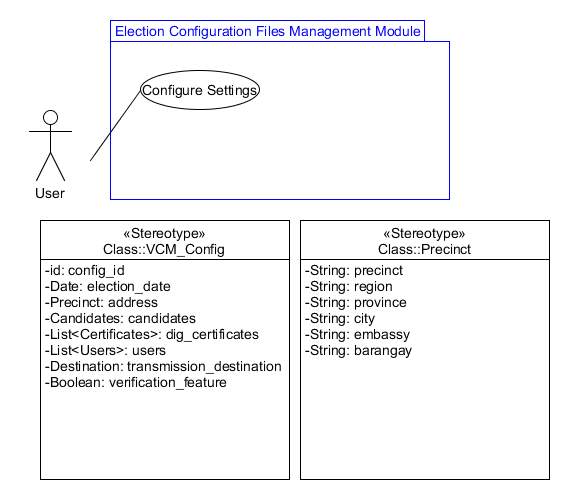
\includegraphics[width=\textwidth]{ecf}
	\end{center}
\end{figure}
\subsubsection*{Ballot Definition Management Module}
\begin{figure}[H]
	\begin{center}
		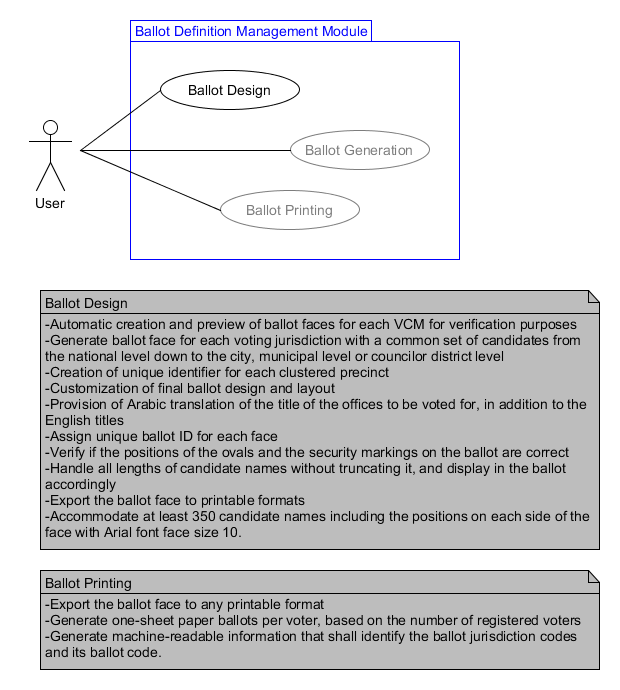
\includegraphics[width=\textwidth]{bdef}
	\end{center}
\end{figure}
\subsubsection*{Machine Configuration Management Module}
\begin{figure}[H]
	\begin{center}
		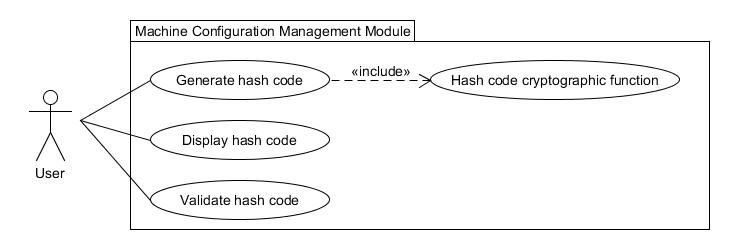
\includegraphics[width=\textwidth]{mc1}
		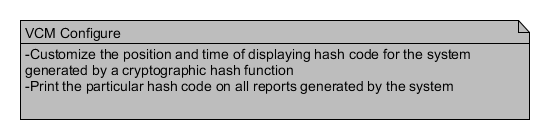
\includegraphics[width=0.8\textwidth]{mc}
	\end{center}
\end{figure}
\subsubsection*{Election Data Report Format Management Module}
\begin{figure}[H]
	\begin{center}
		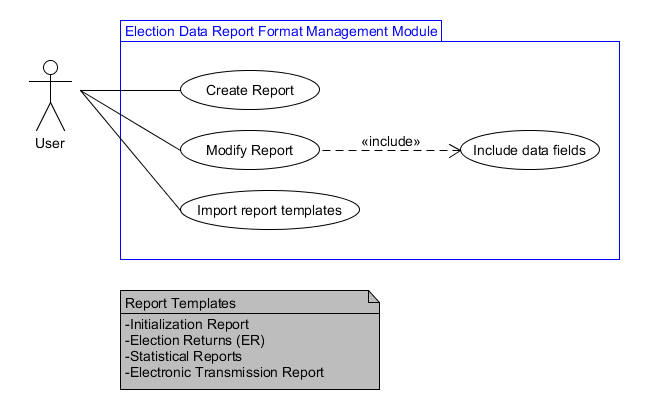
\includegraphics[width=\textwidth]{report}
	\end{center}
\end{figure}


\section{Non-Functional Requirements}
This section outlines general system requirements that are applicable to the EMS, VCM and OMR.

\subsection{General Requirements}
\begin{itemize}
	\item The overall system shall establish a core, web-based data storage and retrieval system to support the consolidation of election data as well as the dissemination of this information among the relevant audience.
	\item The system shall be designed for unattended operation under normal circumstances, exclusive of manual data entry, public user access, and routine administrative functions.
\end{itemize}

\subsection{Availability and Reliability}
\begin{itemize}
	\item The system shall be designed to achieve persistent ("always on") availability.
	\item Administrative and maintenance activities that require the web application to be down can be at off-peak times (non-office hours) to maximize system availability for public users.
	\item The web application shall be complemented with large and secure storage and shall respond most user queries within least time while supporting 2000 machines and 16 million users on real-time conditions.
\end{itemize}
To ensure availability of service, the system should be tested in different setup environments and weather conditions. For reliability, unit testing up to systems integration testing should be done together with the user acceptance conditions to ensure it will deliver the expected results.

\subsection{Expandability and Scalability}
\begin{itemize}
	\item The overall system shall be designed with an open architecture intended to facilitate addition of functionality and scale of the system as new data sources, functionalities and technologies may come in the future.
	\item Object-oriented design is implemented to facilitate modification of the individual modules of the system without affecting the whole system.
\end{itemize}

\subsection{Security and Privacy}
\begin{itemize}
	\item The database, hardware, software, communications and other peripherals shall be protected in accordance with state-of-the-art security precautions to guard against intentional and non-intentional threats to the integrity of the system from unauthorized access, malicious scripts, and other sources of potential harm.
	\item The system shall use access control privileges to access data based on a user's role (e.g. administrator, election offices, etc.).
\end{itemize}
In addition to mentioned above, the overall system will also implement up-to-date security tools:
\begin{itemize}
	\item Elliptic curve cryptography (ECC) with random salt so that the recovery of original passwords is nearly impossible.
	\item Secure Sockets Layer (SSL) to encrypt the data coming to or from the machines and prevent man-in-the-middle attacks.
	\item Burp Suite to eradicate all vulnerabilities of the web-based system like cookie hijacking, cross-site request forgery and cross-site scripting.
\end{itemize}
Lastly, the system will be subject to comprehensive penetration testing to fulfill the security and privacy aspects.

\subsection{Audit Log}
All activities in the system including user, errors, warnings should be written in audit logs for future reference. Logs are also used to verify the correctness of the system. Audit logs contain the following information:
\begin{itemize}
	\item Unique EMS machine ID currently used by a particular user
	\item Information about the unique ID of the user
	\item Specific date and time of the logged event
	\item Specific type of event whether system activity, user activity or errors
	\item Specific access and action done on EMS records
\end{itemize}
Specific changes on the logs done outside the system shall be detected.

\subsection{Performance}
The functionalities of each system is subject to benchmarking in terms of time and space consumption to maximize its performance.
The web framework that will be used has its own benchmarking tools, aside from the developer tools of Google Chrome browser.

\subsection{Error Handling and Monitoring}
\begin{itemize}
	\item The system shall include tools to allow for automatic detection and handling of system errors.
	\item The system shall automatically notify the administrator when errors have occurred through detailed on-screen warning messages.
	\item All system errors, warnings, and recovery actions shall be recorded in an exportable ASCII text file system audit log.
	\item The system shall incorporate automatic shut down and restart features that preserve system integrity and minimizes potential damage in the event of power failures.
\end{itemize}
The system should be tested on all use cases, erroneous user inputs, functionalities and tendencies to system errors.

\subsection{Backup and Recovery}
The systems allows export of all data in MySQL or CSV file formats. Back-up of data is also included for data recovery purposes. Data recovery is automatic: user does not have to manually regenerate missing files to continue working on the systems.

\subsection{Knowledge Transfer}
All software, hardware, instructional materials and comprehensive documentation of source codes shall be turned over to COMELEC after the project. The COMELEC can also modify the system for its own purposes.

\section{Risk Management}
\subsection{Purpose and Objectives}
Risk Management is the systematic process of identifying, analyzing, and responding to project risks. It includes maximizing the probability and consequences of positive events and minimizing the probability and consequences of adverse effects to project objectives. A risk management plan defined how a project team will handle risks to achieve that goal.
\subsubsection{Risk}
An uncertain event or condition that, if it occurs, has a positive or negative effect on a project's objectives. Risk is ofter a measure of the inability to achieve overall project objectives within defiend project requirements and constraints and has three components:
\begin{enumerate}
	\item probability of occurrence
	\item impact of the risk on the program
	\item time horizon during which the consequences will occur if the risk is not mitigated
\end{enumerate}

\subsubsection{Probability of Occurence and Risk Impact}
The following table defines the probability of occurrence.
\begin{figure}[H]
	\begin{center}
		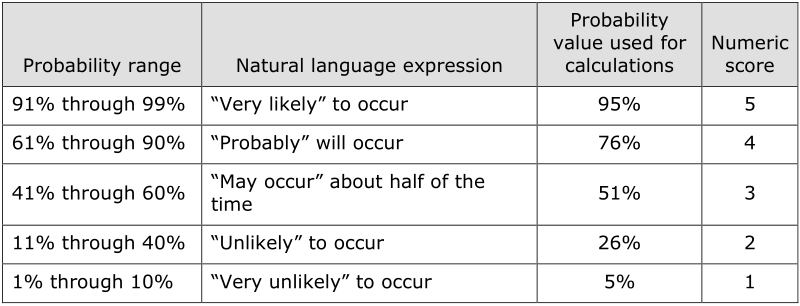
\includegraphics[width=\textwidth]{prob}
	\end{center}
\end{figure}
The following table defines the risk impact categories and terms. For positive risks, consider the the opposite of the impact description. The examples would remain the same except having a positive impact to the project.
\begin{figure}[H]
	\begin{center}
		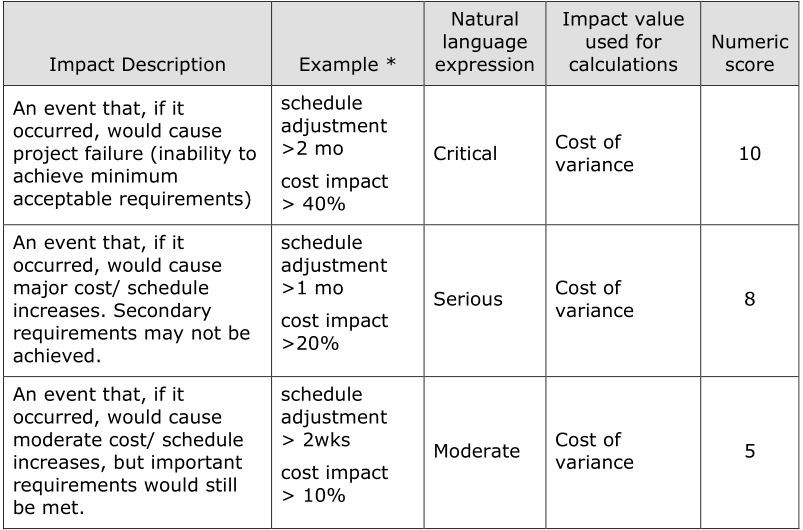
\includegraphics[width=\textwidth]{risk}
		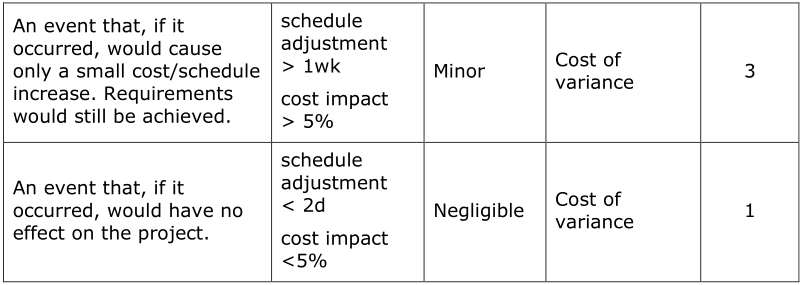
\includegraphics[width=\textwidth]{risk2}
	\end{center}
\end{figure}

\subsubsection{Risk Score}
The risk score is a value calculated that is the product of probability of occurrence and impact. You use the score to compare risks as part of the risk prioritization process. The table \ref{tbl:matrix} is the matrix used to develop the risk score. The values range from 1 (very low exposure) to 50 (very high exposure). Although there are no specific break points in the risk exposure ranking, those risks with an exposure value between 20 and 39 are considered moderate risks, and those risks with an exposure value between 40 and 50 are considered high risks. The definitions of Low, Moderate and High are as follows:
\begin{itemize}
	\item \textbf{Low Risk}: Has little or no potential for increase in cost, disruption of schedule, or degradation of performance. Actions within the scope of the planned project and normal management attention should result in controlling acceptable risk. No response plans will be amde for these risks. The project will monitor for them and manage them as they come up.
	\item \textbf{Moderate Risk}: May cause some increase in cost, disruption of schedule, or degradation of performance. Special action and management attention may be required to control acceptable risk. The project will do some response planning for these risks.
	\item \textbf{High Risk}: Likely to cause significant increase in cost, disruption of schedule, or degradation of performance. Significant additional action and high priority management attention will be required to control acceptable risk. The project will do in-depth response plans for these risks.
\end{itemize}
Positive risks can use the same table and descriptions except instead of trying to avoid the risk, we will endeavor to make the risk occur and gain the positive impact.
\begin{figure}[H]\label{fig:matrix}
	\begin{center}
		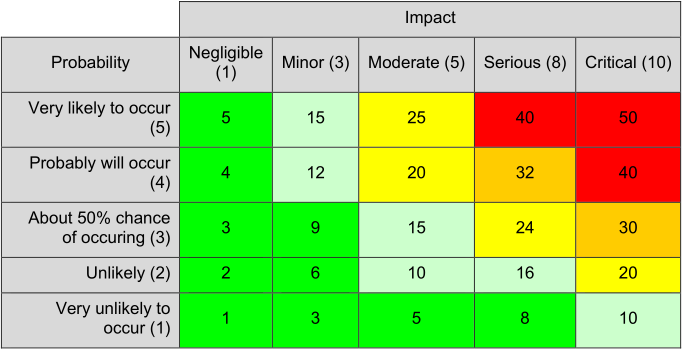
\includegraphics[width=\textwidth]{matrix}
		\caption{Risk Score Matrix}
	\end{center}
\end{figure}

\subsection{Organization}
This section defines the roles and responsibilities for risk management.
\subsubsection{Roles and Responsibilities}
\begin{figure}[H]
	\begin{center}
		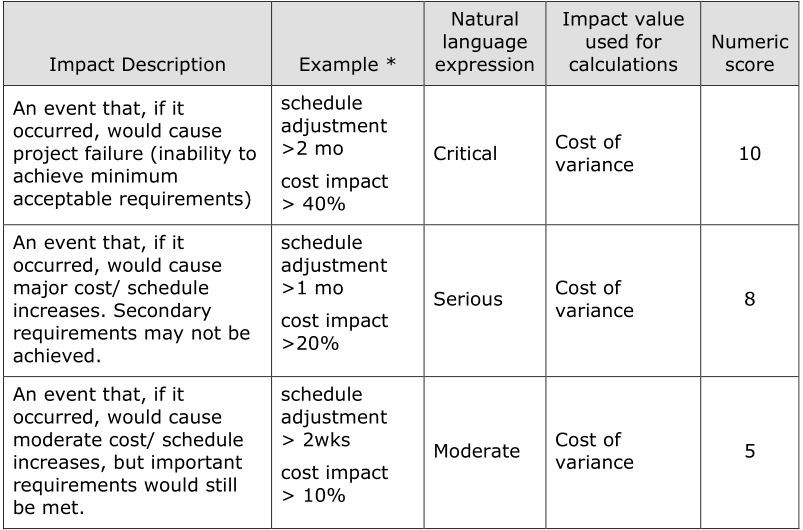
\includegraphics[width=\textwidth]{risk}
		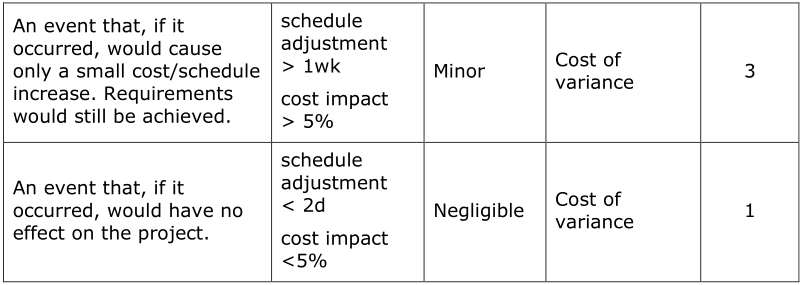
\includegraphics[width=\textwidth]{risk2}
	\end{center}
\end{figure}

\subsection{Risk Management Structure and Procedures}
This section describes the risk management process and provides an overview of the risk management approach.
\subsubsection{Risk Assessment}
\begin{itemize}
	\item \textbf{Size:} With a budget of Php 2,503,518,000.00, this project is a large-scale project to implemented nationwide.
	\item \textbf{Complexity:} This project involves multiple divisions within the organization, but does not involve any other agency or external organization. The project does work with complex election system with dedicated software and hardware for it.  Intercommunication with thousands of dedicated hardwares is also a requirement of this project, together with databases that can handle big data and recovers fast when it encounter errors. Furthermore, this is a critical system and we rate this hard complexity.
	\item \textbf{Importance to Business:} This project is determined to be of high priority within the agency.
	\item \textbf{Visibility:} Relevant information about the project should be hidden to the public. But once completed and deployed, it shall be used by the registered voters of the Philippines.
	\item \textbf{Agency History} Agency rarely does IT projects of this size or complexity.
	\item \textbf{Project Manager (PM): } Agency has its own set pf project managers to manage diverse set of projects.
	\item \textbf{Agency Project Team} About 10\% of the software engineers have done a similar project.
	\item \textbf{Risk Management Effort Decision: } It has been determined that the project will spend full time performing the following risk assessment activities.
\end{itemize}
\subsubsection{Risk Identification}
\begin{enumerate}
	\item \textbf{Brainstorming:} The stakeholders, together with software engineers and testers will be brought in, given a brief overview of the project, then, using the brainstorming technique, they will be asked to identify any opportunities they see. We will then ask them to identify any risks. We will ask the group to perform an affinity diagram to categorize the risks and identify any missing risks/opportunities.
	In addition to the above, the core project team will perform a risk breakdown structure (RBS). This involves stepping through the
	Work Breakdown Structure (WBS) task by task and identifying risks \& opportunities associated with the task.
	\item \textbf{Delphi Technique:} We will query software architects to identify risks associated with this project. They will be given a week to respond. After they return all submissions, we will send the total risk list to them for a one-time only review. They will be given an additional week for review/response.
	\item \textbf{Email:} At the end of each of the above activities, everyone will be asked to e-mail the PM with any additional opportunities or risks that occur to them after the session.
\end{enumerate}
The project will use the following categories of risk in this process:
\begin{figure}[H]
	\begin{center}
		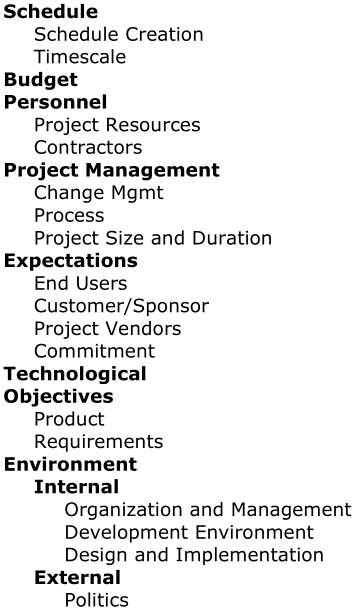
\includegraphics[width=0.4\textwidth]{types}
	\end{center}
\end{figure}

\subsubsection{Qualitative Analysis}
\begin{enumerate}
	\item \textbf{Review:} The PM will ask the core developer and tester teams to review the risks to determine of they understand the risks enough to score. The team should notify the PM of any risk they are unsure of and the PM can clarify or get more information from the originator. The team will have 3 days to perform the review.
	\item \textbf{Scoring:} The project team will determine the
	impact and probability scores for each risk to calculate the risk score. They will use table \ref{fig:matrix} of this document.
	\item \textbf{Threshold 1:} Anything with a probability of "very likely" (5) will be considered a fact and managed in the project plan. \textbf{Threshold 2:} Any thing with a risk score of 20 or below will be included on the non-critical risk list.
	\item All risks not excluded by the above thresholds will be passed to Quantitative Analysis.
	\item \textbf{Stage Gate:} Meet with the Executive Steering 	Committee to review the key risks and get a	go/no-go decision to proceed with planning.
\end{enumerate}

\subsubsection{Quantitative Analysis}
\begin{enumerate}
	\item A moderate risk effort indicates that an Expected Monetary Value (EMV) Analysis will be performed for each of the risked passed onto this phase.
	\item \textbf{Analyze:} The project team and SMEs from the effected divisions will meet to perform a basic EMV for each risk. A decision tree will be developed for a risk as needed.
\end{enumerate}

\subsubsection{Risk Response Planning}
\begin{enumerate}
	\item The top risks evaluated in the Quantitative Analysis will be assigned out to the core project team, SMEs, and management if
	necessary. Each risk owner will be assigned to develop strategies avoid, if possible, or mitigate/transfer the risk. These responses
	should be documented in the risk register. Risk owners are given 1 week to complete.
	\item \textbf{Stage Gate:} Meet with the Executive Steering 	Committee to review the key risks and get a	go/no-go decision to proceed with planning.
\end{enumerate}

\subsubsection{Risk Monitoring and Control}
\begin{itemize}
\item \textbf{Monitoring:} Risk owners are responsible for monitoring their risks and notifying the PM via e-mail when atrigger occurs and that the response plan has been initiated.
\item \textbf{New Risk identification:} Any stakeholder can identify additional risks. The stakeholder should notify the project manager of the new risk (or possible risk) via e-mail.
\item \textbf{Audits:} The PM will be responsible for overseeing risk activities and ensuring the risk register is updated.
\item \textbf{Review:} The project team will review the project's risks biweekly (in every other weekly team meeting).
\item \textbf{Reporting:} Risks will be reported in two ways. First, the PM maintain a Risk Log in the project repository. The Risk Log will contain a list of risks that are active on the project, the priority of the risk, the assignment, and a current status. Second, the monthly Status Report and the quarterly Large Project Oversight report will contain a summary of the Risk Log and any new risks identified and added to the Risk Register.
\end{itemize}

\subsection{Risk Register}
The project's risk register is located in the project repository and covers the following points.
\begin{itemize}
	\item \textbf{Date Identified:} the date the risk was identified.
	\item \textbf{Status:} identifies whether the risk is potential, active, or closed.
	\item \textbf{Risk Description:} a description of the risk.
	\item \textbf{Risk Probability:} the likelihood that the risk will occur.
	\item \textbf{Risk Impact:} the effect of the project objects if the risk event occurs.
	\item \textbf{Risk Score:} reflects the severity of the risks effect on objectives. The risk score is determined by multiplying the risk probability and risk impact values. The intent is to assign a relative value to the impact on project objectives if the risk in question should occur.
	\item \textbf{Risk Assignment:} person(s) responsible for the risk if it should occur.
	\item \textbf{Agreed Response:} the strategy that is most likely to be effective.
	\begin{itemize}
		\item \textit{Avoidance:} Risk avoidance entails changing the project plan to eliminate the risk or condition or to protect the project objectives from its impact.
		\item \textit{Transference:} Risk transference is seeking to shift the consequence of a risk to a third party together with ownership of the response. Transferring the risk simply gives another party responsibility for its management; it does not eliminate it.
		\item \textit{Mitigation:} Risk mitigation seeks to reduce the probability and/or consequences of an adverse risk event to an acceptable threshold. Taking early action to reduce the probability of a risk or its impact on the project is more effective than trying to repair the	consequences after it occurs.
		\item \textit{Acceptance:} This technique indicates that the project team has decided not to change the project plan to deal with a risk or is unable to identify any other suitable response strategy.
	\end{itemize}
	\item \textbf{Risk Response Plan:} Specific actions to enhance opportunities and reduce threats to the project's objectives.
\end{itemize}

\subsubsection{Identified Risks}
\begin{table}[H]
	\begin{tabular}{l|l l l}
		\textbf{ID} & \textbf{Risk/Event} & \textbf{Status} & \textbf{Probability}\\
		1 & Malfunction of VCM due to workload stress & Potential & 10\% \\
		  & \textbf{Agreed Response} & \textbf{Impact} & \textbf{Est. Risk Cost} \\
		  & Mitigation & Moderate & Php10,000 \\
		  & \textbf{Description} \\
		  & \multicolumn{3}{p{\linewidth}}{Due to different environmental conditions, power sources and stress testing, the VCM may not deliver the results properly and accurately as it was.} \\
		  & \textbf{Assessment} \\
		  & \multicolumn{3}{p{\linewidth}}{Testing of hardware in different weather conditions and workloads shall commence.} \\
		  & \textbf{Response Plan} \\
		  & \multicolumn{3}{p{\linewidth}}{The affected hardware will be replaced/repaired with a working hardware, at no cost on COMELEC.} \\
		  & \textbf{Lessons Learned} \\
		  & The risk has not been active. \\
		\hline
		
		\textbf{ID} & \textbf{Risk/Event} & \textbf{Status} & \textbf{Probability}\\
		2 & Malfunction of EMS due to workload stress & Potential & 5\% \\
		& \textbf{Agreed Response} & \textbf{Impact} & \textbf{Est. Risk Cost} \\
		& Mitigation & Moderate & Php8,000 \\
		& \textbf{Description} \\
		& \multicolumn{3}{p{\linewidth}}{Malfunction of EMS can be in different forms such as database connection errors and web server errors.} \\
		& \textbf{Assessment} \\
		& \multicolumn{3}{p{\linewidth}}{Web based applications deployed in the cloud have a very small probability to malfunction at the server side, since GoDaddy maintains their web servers very well, from databases and server engines. However, they are still subject to testing in different times, peak hours and workload stress to ensure scalability of EMS.} \\
		& \textbf{Response Plan} \\
		& \multicolumn{3}{p{\linewidth}}{Contact the server administrator for certain kinds of errors if these occured in their side. Otherwise, investigate errors in the developer's side or upgrade website subscription plan to get higher capacity, if necessary.} \\
		& \textbf{Lessons Learned} \\
		& The risk has not been active. \\
		\hline
		
		\textbf{ID} & \textbf{Risk/Event} & \textbf{Status} & \textbf{Probability}\\
		3 & Malfunction of EMS due to workload stress & Potential & 20\% \\
		& \textbf{Agreed Response} & \textbf{Impact} & \textbf{Est. Risk Cost} \\
		& Mitigation & Critical & Php1,000,000 \\
		& \textbf{Description} \\
		& \multicolumn{3}{p{\linewidth}}{Shortage of electricity and Internet connection} \\
		& \textbf{Assessment} \\
		& \multicolumn{3}{p{\linewidth}}{The EMS and VCM cannot operate without electricity and Internet connection. The elections will stop temporarily on areas with shortage, especially in Mindanao.} \\
		& \textbf{Response Plan} \\
		& \multicolumn{3}{p{\linewidth}}{Get alternative sources of energy and Internet connection. Use generators or mobile data for the moment.} \\
		& \textbf{Lessons Learned} \\
		& The risk has not been active. \\
	\end{tabular}
\end{table}
\begin{table}[H]
	\begin{tabular}{l| l l l}
		
		\textbf{ID} & \textbf{Risk/Event} & \textbf{Status} & \textbf{Probability}\\
		4 & Natural disasters & Potential & 15\% \\
		& \textbf{Agreed Response} & \textbf{Impact} & \textbf{Est. Risk Cost} \\
		& Acceptance & Serious & Php100,000 \\
		& \textbf{Description} \\
		& \multicolumn{3}{p{\linewidth}}{Unavoidable natural disasters like typhoon, storm surge, fire and earthquake can affect certain utilities like electricity and data connection.} \\
		& \textbf{Assessment} \\
		& \multicolumn{3}{p{\linewidth}}{The national elections will halt on areas affected by natural disasters. Or worse, postpone the national elections on a later date.} \\
		& \textbf{Response Plan} \\
		& \multicolumn{3}{p{\linewidth}}{Place the hardware in strategic places like strong buildings. If such cases happen, save all changes, turn off the hardware immediately.} \\
		& \textbf{Lessons Learned} \\
		& \multicolumn{3}{p{\linewidth}}{Typhoons can be predicted and early warning can be provided. But fires and earthquakes are very unpredictable event.}\\
		\hline
		
		\textbf{ID} & \textbf{Risk/Event} & \textbf{Status} & \textbf{Probability}\\
		5 & Civil War & Potential & 5\% \\
		& \textbf{Agreed Response} & \textbf{Impact} & \textbf{Est. Risk Cost} \\
		& Acceptance & Serious & Php30,000 \\
		& \textbf{Description} \\
		& \multicolumn{3}{p{\linewidth}}{Politically motivated wars can occur in the election day.} \\
		& \textbf{Assessment} \\
		& \multicolumn{3}{p{\linewidth}}{Hardwares can be at risk and can be damaged and destroyed.} \\
		& \textbf{Response Plan} \\
		& \multicolumn{3}{p{\linewidth}}{Place the hardwares in a strategic place where war will least likely to occur, like in the city and town proper.} \\
		& \textbf{Lessons Learned} \\
		& This is a very unpredictable event. \\
		\hline
		\textbf{ID} & \textbf{Risk/Event} & \textbf{Status} & \textbf{Probability}\\
		6 & Unauthorized access to the system & Potential & 20\% \\
		& \textbf{Agreed Response} & \textbf{Impact} & \textbf{Est. Risk Cost} \\
		& Acceptance & Serious & Php30,000 \\
		& \textbf{Description} \\
		& \multicolumn{3}{p{\linewidth}}{Unauthorized users can access the website through social engineering techniques and website penetration.} \\
		& \textbf{Assessment} \\
		& \multicolumn{3}{p{\linewidth}}{Unauthorized access can completely compromise the systems involved including databases, softwares and the like.} \\
		& \textbf{Response Plan} \\
		& \multicolumn{3}{p{\linewidth}}{Place the hardwares in a strategic places with high level of security. If unauthorized access is detected, shut down the system immediately.} \\
		& \textbf{Lessons Learned} \\
		& The risk has not been active.\\
	\end{tabular}
\end{table}

\end{document}
